% Options for packages loaded elsewhere
\PassOptionsToPackage{unicode}{hyperref}
\PassOptionsToPackage{hyphens}{url}
%
\documentclass[
  man]{apa6}
\usepackage{amsmath,amssymb}
\usepackage{iftex}
\ifPDFTeX
  \usepackage[T1]{fontenc}
  \usepackage[utf8]{inputenc}
  \usepackage{textcomp} % provide euro and other symbols
\else % if luatex or xetex
  \usepackage{unicode-math} % this also loads fontspec
  \defaultfontfeatures{Scale=MatchLowercase}
  \defaultfontfeatures[\rmfamily]{Ligatures=TeX,Scale=1}
\fi
\usepackage{lmodern}
\ifPDFTeX\else
  % xetex/luatex font selection
\fi
% Use upquote if available, for straight quotes in verbatim environments
\IfFileExists{upquote.sty}{\usepackage{upquote}}{}
\IfFileExists{microtype.sty}{% use microtype if available
  \usepackage[]{microtype}
  \UseMicrotypeSet[protrusion]{basicmath} % disable protrusion for tt fonts
}{}
\makeatletter
\@ifundefined{KOMAClassName}{% if non-KOMA class
  \IfFileExists{parskip.sty}{%
    \usepackage{parskip}
  }{% else
    \setlength{\parindent}{0pt}
    \setlength{\parskip}{6pt plus 2pt minus 1pt}}
}{% if KOMA class
  \KOMAoptions{parskip=half}}
\makeatother
\usepackage{xcolor}
\usepackage{graphicx}
\makeatletter
\def\maxwidth{\ifdim\Gin@nat@width>\linewidth\linewidth\else\Gin@nat@width\fi}
\def\maxheight{\ifdim\Gin@nat@height>\textheight\textheight\else\Gin@nat@height\fi}
\makeatother
% Scale images if necessary, so that they will not overflow the page
% margins by default, and it is still possible to overwrite the defaults
% using explicit options in \includegraphics[width, height, ...]{}
\setkeys{Gin}{width=\maxwidth,height=\maxheight,keepaspectratio}
% Set default figure placement to htbp
\makeatletter
\def\fps@figure{htbp}
\makeatother
\setlength{\emergencystretch}{3em} % prevent overfull lines
\providecommand{\tightlist}{%
  \setlength{\itemsep}{0pt}\setlength{\parskip}{0pt}}
\setcounter{secnumdepth}{-\maxdimen} % remove section numbering
% Make \paragraph and \subparagraph free-standing
\makeatletter
\ifx\paragraph\undefined\else
  \let\oldparagraph\paragraph
  \renewcommand{\paragraph}{
    \@ifstar
      \xxxParagraphStar
      \xxxParagraphNoStar
  }
  \newcommand{\xxxParagraphStar}[1]{\oldparagraph*{#1}\mbox{}}
  \newcommand{\xxxParagraphNoStar}[1]{\oldparagraph{#1}\mbox{}}
\fi
\ifx\subparagraph\undefined\else
  \let\oldsubparagraph\subparagraph
  \renewcommand{\subparagraph}{
    \@ifstar
      \xxxSubParagraphStar
      \xxxSubParagraphNoStar
  }
  \newcommand{\xxxSubParagraphStar}[1]{\oldsubparagraph*{#1}\mbox{}}
  \newcommand{\xxxSubParagraphNoStar}[1]{\oldsubparagraph{#1}\mbox{}}
\fi
\makeatother
% definitions for citeproc citations
\NewDocumentCommand\citeproctext{}{}
\NewDocumentCommand\citeproc{mm}{%
  \begingroup\def\citeproctext{#2}\cite{#1}\endgroup}
\makeatletter
 % allow citations to break across lines
 \let\@cite@ofmt\@firstofone
 % avoid brackets around text for \cite:
 \def\@biblabel#1{}
 \def\@cite#1#2{{#1\if@tempswa , #2\fi}}
\makeatother
\newlength{\cslhangindent}
\setlength{\cslhangindent}{1.5em}
\newlength{\csllabelwidth}
\setlength{\csllabelwidth}{3em}
\newenvironment{CSLReferences}[2] % #1 hanging-indent, #2 entry-spacing
 {\begin{list}{}{%
  \setlength{\itemindent}{0pt}
  \setlength{\leftmargin}{0pt}
  \setlength{\parsep}{0pt}
  % turn on hanging indent if param 1 is 1
  \ifodd #1
   \setlength{\leftmargin}{\cslhangindent}
   \setlength{\itemindent}{-1\cslhangindent}
  \fi
  % set entry spacing
  \setlength{\itemsep}{#2\baselineskip}}}
 {\end{list}}
\usepackage{calc}
\newcommand{\CSLBlock}[1]{\hfill\break\parbox[t]{\linewidth}{\strut\ignorespaces#1\strut}}
\newcommand{\CSLLeftMargin}[1]{\parbox[t]{\csllabelwidth}{\strut#1\strut}}
\newcommand{\CSLRightInline}[1]{\parbox[t]{\linewidth - \csllabelwidth}{\strut#1\strut}}
\newcommand{\CSLIndent}[1]{\hspace{\cslhangindent}#1}
\ifLuaTeX
\usepackage[bidi=basic]{babel}
\else
\usepackage[bidi=default]{babel}
\fi
\babelprovide[main,import]{english}
% get rid of language-specific shorthands (see #6817):
\let\LanguageShortHands\languageshorthands
\def\languageshorthands#1{}
% Manuscript styling
\usepackage{upgreek}
\captionsetup{font=singlespacing,justification=justified}

% Table formatting
\usepackage{longtable}
\usepackage{lscape}
% \usepackage[counterclockwise]{rotating}   % Landscape page setup for large tables
\usepackage{multirow}		% Table styling
\usepackage{tabularx}		% Control Column width
\usepackage[flushleft]{threeparttable}	% Allows for three part tables with a specified notes section
\usepackage{threeparttablex}            % Lets threeparttable work with longtable

% Create new environments so endfloat can handle them
% \newenvironment{ltable}
%   {\begin{landscape}\centering\begin{threeparttable}}
%   {\end{threeparttable}\end{landscape}}
\newenvironment{lltable}{\begin{landscape}\centering\begin{ThreePartTable}}{\end{ThreePartTable}\end{landscape}}

% Enables adjusting longtable caption width to table width
% Solution found at http://golatex.de/longtable-mit-caption-so-breit-wie-die-tabelle-t15767.html
\makeatletter
\newcommand\LastLTentrywidth{1em}
\newlength\longtablewidth
\setlength{\longtablewidth}{1in}
\newcommand{\getlongtablewidth}{\begingroup \ifcsname LT@\roman{LT@tables}\endcsname \global\longtablewidth=0pt \renewcommand{\LT@entry}[2]{\global\advance\longtablewidth by ##2\relax\gdef\LastLTentrywidth{##2}}\@nameuse{LT@\roman{LT@tables}} \fi \endgroup}

% \setlength{\parindent}{0.5in}
% \setlength{\parskip}{0pt plus 0pt minus 0pt}

% Overwrite redefinition of paragraph and subparagraph by the default LaTeX template
% See https://github.com/crsh/papaja/issues/292
\makeatletter
\renewcommand{\paragraph}{\@startsection{paragraph}{4}{\parindent}%
  {0\baselineskip \@plus 0.2ex \@minus 0.2ex}%
  {-1em}%
  {\normalfont\normalsize\bfseries\itshape\typesectitle}}

\renewcommand{\subparagraph}[1]{\@startsection{subparagraph}{5}{1em}%
  {0\baselineskip \@plus 0.2ex \@minus 0.2ex}%
  {-\z@\relax}%
  {\normalfont\normalsize\itshape\hspace{\parindent}{#1}\textit{\addperi}}{\relax}}
\makeatother

\makeatletter
\usepackage{etoolbox}
\patchcmd{\maketitle}
  {\section{\normalfont\normalsize\abstractname}}
  {\section*{\normalfont\normalsize\abstractname}}
  {}{\typeout{Failed to patch abstract.}}
\patchcmd{\maketitle}
  {\section{\protect\normalfont{\@title}}}
  {\section*{\protect\normalfont{\@title}}}
  {}{\typeout{Failed to patch title.}}
\makeatother

\usepackage{xpatch}
\makeatletter
\xapptocmd\appendix
  {\xapptocmd\section
    {\addcontentsline{toc}{section}{\appendixname\ifoneappendix\else~\theappendix\fi: #1}}
    {}{\InnerPatchFailed}%
  }
{}{\PatchFailed}
\makeatother
\keywords{graphical representation, iconicity, analogy, symbol, communication, emerging literacy\newline\indent Word count: Child Development Max 40 pages // PNAS 1,500–2,000 words}
\DeclareDelayedFloatFlavor{ThreePartTable}{table}
\DeclareDelayedFloatFlavor{lltable}{table}
\DeclareDelayedFloatFlavor*{longtable}{table}
\makeatletter
\renewcommand{\efloat@iwrite}[1]{\immediate\expandafter\protected@write\csname efloat@post#1\endcsname{}}
\makeatother
\usepackage{lineno}

\linenumbers
\usepackage{csquotes}
\ifLuaTeX
  \usepackage{selnolig}  % disable illegal ligatures
\fi
\usepackage{bookmark}
\IfFileExists{xurl.sty}{\usepackage{xurl}}{} % add URL line breaks if available
\urlstyle{same}
\hypersetup{
  pdftitle={Young children's spontaneous comprehension of symbol-object-relationships in the graphic domain},
  pdfauthor={Gregor Kachel1, Daniel Haun2, \& Manuel Bohn1},
  pdflang={en-EN},
  pdfkeywords={graphical representation, iconicity, analogy, symbol, communication, emerging literacy},
  hidelinks,
  pdfcreator={LaTeX via pandoc}}

\title{Young children's spontaneous comprehension of symbol-object-relationships in the graphic domain}
\author{Gregor Kachel\textsuperscript{1}, Daniel Haun\textsuperscript{2}, \& Manuel Bohn\textsuperscript{1}}
\date{}


\shorttitle{Comprehension of symbol-object-relationships}

\authornote{

\emph{Ethics, consent and conflict of interest}: This study confirms with recognized standards (e.g.~the Declaration of Helsinki) and was approved by an internal ethics committee at the Max-Planck-Institute for Evolutionary Anthropology. Informed consent has been obtained from all participants. The authors declare no conflict of interest.

\emph{Acknowledgments}: We are thankful to Susanne Mauritz for her help in the organization of the study and to Valerie Jurgenson and Cynthia Pones for help with data collection. We would like to thank Anne Deiglmayr for hosting this project in her research group and for her continuous support. Finally, we are very thankful to all parents and children participating in the study. Gregor Kachel was supported by the German Research Foundation (Deutsche Forschungsgemeinschaft) under project number 429220405.

The authors made the following contributions. Gregor Kachel: Conceptualization, Funding Acquisition, Project Administration, Investigation, Methodology, Data Curation, Formal Analysis, Visualization, Writing - Original Draft Preparation, Writing - Review \& Editing; Daniel Haun: Resources, Writing - Review \& Editing; Manuel Bohn: Methodology, Software, Formal Analysis, Validation, Writing - Review \& Editing, Supervision.

Correspondence concerning this article should be addressed to Gregor Kachel, Universitätsallee 1, C1.008a, 21335 Lüneburg. E-mail: \href{mailto:gregor.kachel@leuphana.de}{\nolinkurl{gregor.kachel@leuphana.de}}

}

\affiliation{\vspace{0.5cm}\textsuperscript{1} Leuphana University\\\textsuperscript{2} Max-Planck-Institute for Evolutionary Anthropology}

\abstract{%
One or two sentences providing a \textbf{basic introduction} to the field, comprehensible to a scientist in any discipline.
Two to three sentences of \textbf{more detailed background}, comprehensible to scientists in related disciplines.
One sentence clearly stating the \textbf{general problem} being addressed by this particular study.
One sentence summarizing the main result (with the words ``\textbf{here we show}'' or their equivalent).
Two or three sentences explaining what the \textbf{main result} reveals in direct comparison to what was thought to be the case previously, or how the main result adds to previous knowledge.
One or two sentences to put the results into a more \textbf{general context}.
Two or three sentences to provide a \textbf{broader perspective}, readily comprehensible to a scientist in any discipline. !Abstract must be less then 120words!
}



\begin{document}
\maketitle

\section{Introduction}\label{introduction}

Lorem ipsum dolor sit amet, consetetur sadipscing elitr, sed diam nonumy eirmod tempor invidunt ut labore et dolore magna aliquyam erat, sed diam voluptua. At vero eos et accusam et justo duo dolores et ea rebum. Stet clita kasd gubergren, no sea takimata sanctus est Lorem ipsum dolor sit amet. Lorem ipsum dolor sit amet, consetetur sadipscing elitr, sed diam nonumy eirmod tempor invidunt ut labore et dolore magna aliquyam erat, sed diam voluptua. At vero eos et accusam et justo duo dolores et ea rebum. Stet clita kasd gubergren, no sea takimata sanctus est Lorem ipsum dolor sit amet.

\emph{General notes Citing stuff}. You have to make sure that the respective reference in included in the bib-file. I would also suggest to have two additional folders in the root, namely (1) papers to cite - where we can dumb pdfs, and (2) papers\_cited. Whenever you are adding a new reference please put the citation in bibtex, name the pdf accorind to the bibtext id and add the pdf to the papers\_cited folder. And this is how to cite something in markdown: Preschoolers invent and comprehend iconic gestures spontaneously (Bohn, Kachel, \& Tomasello, 2019).

\emph{Children's understanding of graphical representations}. Lorem ipsum dolor sit amet, consetetur sadipscing elitr, sed diam nonumy eirmod tempor invidunt ut labore et dolore magna aliquyam erat, sed diam voluptua. At vero eos et accusam et justo duo dolores et ea rebum. Stet clita kasd gubergren, no sea takimata sanctus est Lorem ipsum dolor sit amet. Lorem ipsum dolor sit amet, consetetur sadipscing elitr, sed diam nonumy eirmod tempor invidunt ut labore et dolore magna aliquyam erat, sed diam voluptua. At vero eos et accusam et justo duo dolores et ea rebum. Stet clita kasd gubergren, no sea takimata sanctus est Lorem ipsum dolor sit amet.

\emph{This Paper}. Lorem ipsum dolor sit amet, consetetur sadipscing elitr, sed diam nonumy eirmod tempor invidunt ut labore et dolore magna aliquyam erat, sed diam voluptua. At vero eos et accusam et justo duo dolores et ea rebum. Stet clita kasd gubergren, no sea takimata sanctus est Lorem ipsum dolor sit amet. Lorem ipsum dolor sit amet, consetetur sadipscing elitr, sed diam nonumy eirmod tempor invidunt ut labore et dolore magna aliquyam erat, sed diam voluptua. At vero eos et accusam et justo duo dolores et ea rebum. Stet clita kasd gubergren, no sea takimata sanctus est Lorem ipsum dolor sit amet. For the first time, the studies contributing to this paper investigate children's understanding of xxx.

\emph{Hypotheses}. Lorem ipsum dolor sit amet, consetetur sadipscing elitr, sed diam nonumy eirmod tempor invidunt ut labore et dolore magna aliquyam erat, sed diam voluptua. At vero eos et accusam et justo duo dolores et ea rebum. Stet clita kasd gubergren, no sea takimata sanctus est Lorem ipsum dolor sit amet. Lorem ipsum dolor sit amet, consetetur sadipscing elitr, sed diam nonumy eirmod tempor invidunt ut labore et dolore magna aliquyam erat, sed diam voluptua. At vero eos et accusam et justo duo dolores et ea rebum. Stet clita kasd gubergren, no sea takimata sanctus est Lorem ipsum dolor sit amet.

\section{Methods}\label{methods}

All three studies below share the same basic methods and analyses. For convenience, common aspects of the procedure, participant recruiting and stimulus design are reported first before discussing the indivual studies respectively.

\subsection{General Methods}\label{general-methods}

\subsubsection{Setup and Data Collection}\label{setup-and-data-collection}

Children were visited in-person at their daycares. Daycares provided a separate room where experimenters (E) and children watched the presentation of a picture-book like hiding game on screen while sitting at their side. See figure \ref{fig:figure-setup} for an illustration of the setup.

See figure XXX for an illustration of the setup.



\begin{figure}

{\centering 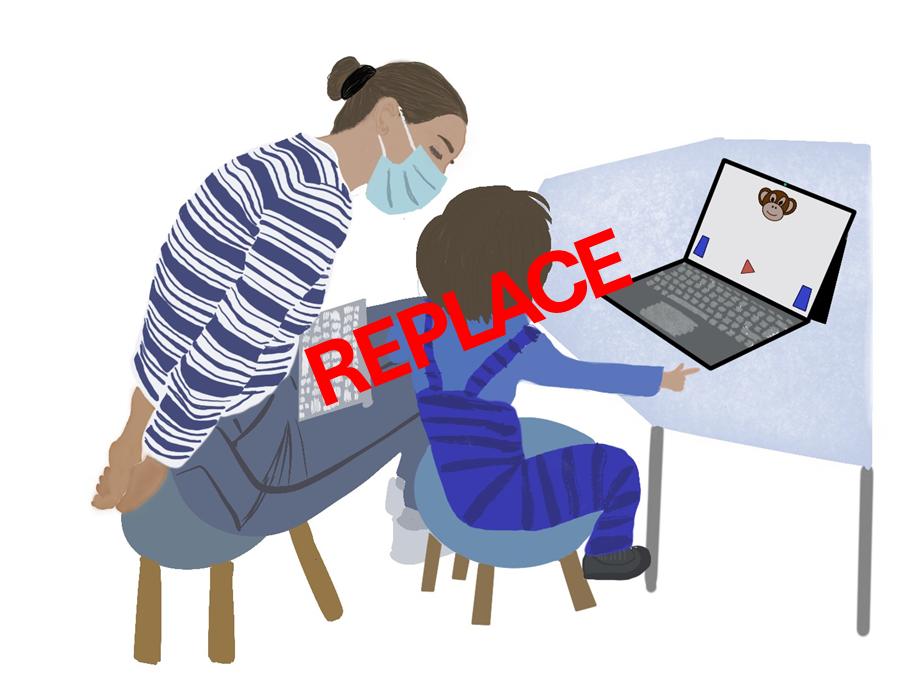
\includegraphics{../illustrations/Symlit_Rep_Setup} 

}

\caption{Illustration of setup.}\label{fig:figure-setup}
\end{figure}

\subsubsection{Procedure}\label{procedure}

\emph{Familiarization}.

E introduced an agent, namely a cartoon monkey, and familiarized children with the framing of the task. The monkey placed two small cups at the bottom of the screen. Next, the cups were lifted and the monkey dropped a banana under one of them. The cups were lowered again to hide the banana. Hence, children saw an item being hidden in plain sight and were solely required to remember its place for a minimal amount of time before being asked ``Where is the banana?''. Children were required to point at the correct hiding place. In the familiarization phase, children received immediate feedback from the experimenter (``Well done!'' / ``hmm, lets go again!'') while the hiding place of the banana was revealed.

To ensure that children were familiar with the goal of the game and the touch interface, they first had to complete a set of four to eight familiarization trials with a success rate of 75\%. In case a child did not reply correctly in three out of four trials, another four familiarization trials were provided. If the child was correct in six out of eight trials, she was included in the main sample. Children that did not succeed during familiarization were allowed to participate further but their data was not submitted to analysis.

\emph{Test phase}. The main phase of the study commenced with announcing that the cartoon character had an idea for a new game.

E explains that they must not see where the banana is hidden. The hiding sequence is identical to the familiarization phase, however the placement of the banana is covered by a wood fence over the lower half of the screen. Next, the monkey holds up piece of paper and a pen

The hiding place is not revealed and children do not receive feedback in test trials. E acknowledges their choices by thanking them in a neutral tone and moves on to the next trial.

Except for the geometric shapes and their placement, the presentations in both conditions were identical. A single trial lasted 20 to 30 seconds. Children were presented with 16 test trials containing the four test conditions in a blocked order.

In order to be submitted to the analyses participants had to complete at least eight valid test trials (see coding below).The entire test sessions lasted about 12 minutes.

\subsubsection{Stimuli}\label{stimuli}

Description of cues and targets and maybe how they were created. For an illustration of the stimuli and example presentations, please see supplementary materials sections XX and XX.

\subsubsection{Data Handling and Analyses}\label{data-handling-and-analyses}

Participant responses were collected directly by the experimental script

Bayesian models were run in Stan (\url{http://mc-stan.org/}) and implemented via the function brm of the package brms (Bürkner, 2017). We used logistic Bayesian generalized linear mixed models (GLMM) to fit children's responses (0/1) as a function of their absolute age in days, condition (rep, pars, fsim, fcom) and an interaction between trial and task. We use default priors and include trial and sex as fixed effects to be controlled for. Trial number will be added as a random slope within subject.

The full model notation was: \('correct~condition*z.age+z.trial+z.sex+(z.trial|subid)'\)
• correct: correct choice (0/1)
• z.age: age in days, centered to a mean of 0
• z.trial: trial number, scaled
• z.sex: participants' sex (male/female), scaled

The analysis modeled participants binary choices to predict the probability of children interpreting the cues correctly and model how this probability will change as a function of their absolute age in days. We used the model to predict the
developmental trajectory (with 95\% CrI) for each task type. The criterion for settling when children perform above chance with either type of stimuli is the point at which the 95\% CrI for a particular trajectory does no longer overlap with a midline demarcating the 50\% chance level.

For our main analyses, we used logistic Bayesian generalized linear mixed models (GLMM) to fit children's responses (0/1) as a function of their absolute age in days, task (arrow, marker) and an interaction between trial and task. We used default priors and included trial and sex as fixed effects to be controlled for. Trial number was added as a random slope within subject. The full model notation was \('correct ~ task*z.age +z.trial +z.sex +(z.trial|id)'\).

The analysis models participants binary choices to predict the probability of children interpreting the cues correctly and model how this probability will change as a function of their absolute age in days. In order to evaluate the relevance of age and task type for children's performance, we compared a full model as specified above with a reduced model lacking the interaction of age and task by using WAIC scores and weights (McElreath, 2016). Furthermore, we inspected the model estimates for the different predictors (including their 95\% Credible Interval (CrI)). To answer our main research question of when children perform above chance in a task, we use the model to predict the developmental trajectory (with 95\% CrI) for each task type. The criterion for settling when children perform above chance is the point at which the 95\% CrI for a particular trajectory does no longer overlap with a midline demarcating the 50\% chance level.

To further explore our data, we also binned participants in age-groups (three-, and four-year-olds). To test whether group-level performance was above chance in all experimental groups, we used two-tailed one-sample t-tests with the chance level set to .5. We provide Cohen's d as a standardized effect size for significance testing (computed via the function \texttt{cohensD}). Additionally, each participant's data was also submitted to a binomial test to determine whether their performance was above chance on an individual level.

\subsection{Study 1}\label{study-1}

\subsubsection{Participants}\label{participants}

In order to model children's development across the preschool years continuously while aligning with conventions in the field, data collection aimed at testing two children per month of age between the third and the seventh birthday for a minimum of 96 participants (24 per year). As children were tested on the basis of availability, the final sample exceeds this preregistered minimum by ten participants. The final sample consisted of 106 children (M = 59.18 months, SD = 13.58 months, range 36 - 83 months; 51 female). In addition, 22 children (11 female) were tested but excluded from analysis for not succeeding during familiarization (N = 13), for not completing at least eight out of 16 test trials (N = 1), or due to being fussy (N = 2). For 4 children, experimenters only learned during testing that children were not fluent enough in German to participate as their families had only recently migrated. Finally, 2 children had to be excluded due to technical issues. For a graphical and tabular overview of participants and exclusions across all three studies presented here, please see Appendix A.

All participants were recruited in \textbf{MASKED FOR REVIEW}, a medium-sized middle-European city, and came from a predominantly white population of middle to high income families. They were contacted via a database of participants for child development studies to which their parents had voluntarily signed up. Appointments were made on the basis of parents' and children's availability. The study was reviewed and approved by an internal ethics committee at the \textbf{MASKED FOR REVIEW}. Data collection took place from June 2022 to February 2023.

\subsubsection{Stimuli}\label{stimuli-1}

\subsubsection{Analyses}\label{analyses}

\subsubsection{Results}\label{results}

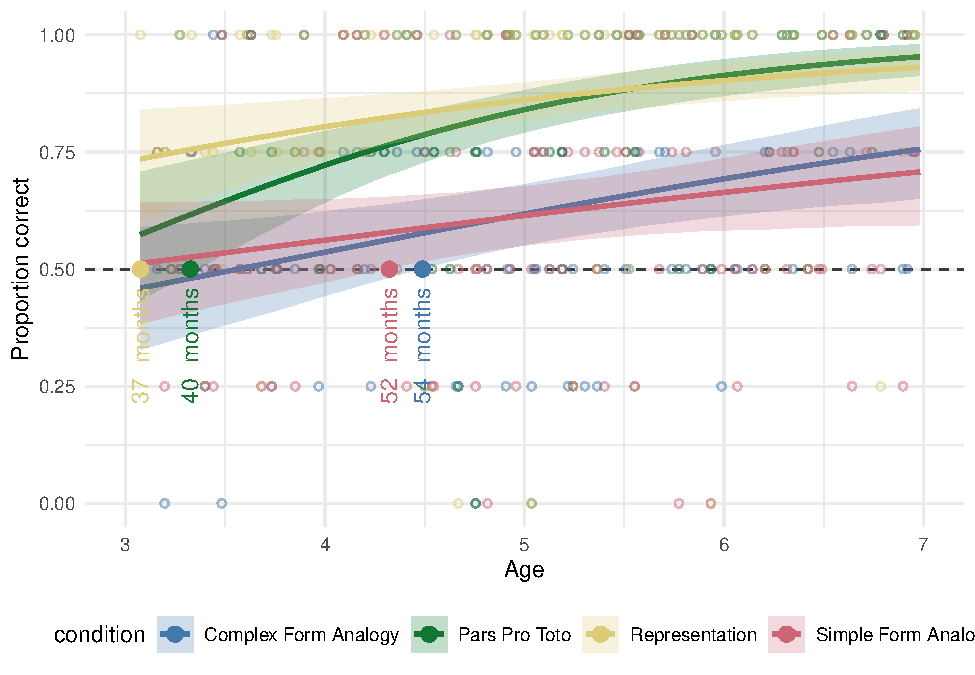
\includegraphics{symlit_rep_manuscript_files/figure-latex/S1_bayes_plot_no_facets-1.pdf}

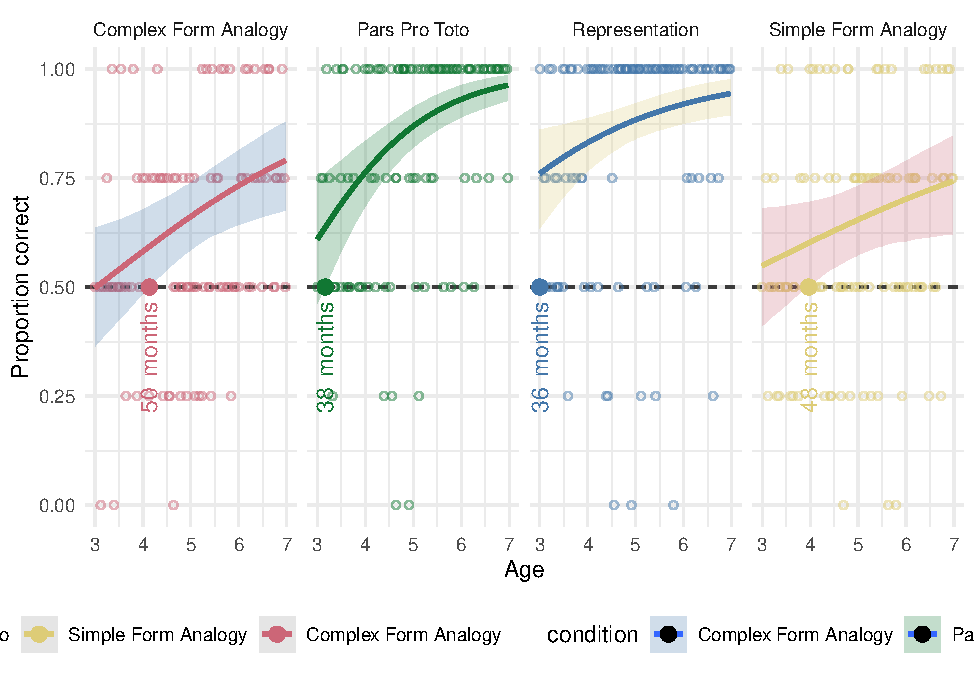
\includegraphics{symlit_rep_manuscript_files/figure-latex/S1_bayes_plot-1.pdf}

Lorem ipsum dolor sit amet, consetetur sadipscing elitr, sed diam nonumy eirmod tempor invidunt ut labore et dolore magna aliquyam erat, sed diam voluptua. At vero eos et accusam et justo duo dolores et ea rebum. Stet clita kasd gubergren, no sea takimata sanctus est Lorem ipsum dolor sit amet. Lorem ipsum dolor sit amet, consetetur sadipscing elitr, sed diam nonumy eirmod tempor invidunt ut labore et dolore magna aliquyam erat, sed diam voluptua. At vero eos et accusam et justo duo dolores et ea rebum. Stet clita kasd gubergren, no sea takimata sanctus est Lorem ipsum dolor sit amet.

\subsection{Study 2}\label{study-2}

\subsubsection{Participants}\label{participants-1}

A total of 99 three- to seven-year-old children (M = 60.04 months, SD = 13.69 months, range 36 - 83 months; 49 female) participated. In addition, 15 children (7 female) were tested but excluded from analysis for failing familiarization (N = 10), being fussy (N = 2), not being fluent in German (N = 1) or due to technical issues (N = 2).

\subsubsection{Materials}\label{materials}

\subsubsection{Data analysis}\label{data-analysis}

Notation
Evaluation of model Stability

\subsubsection{Results}\label{results-1}

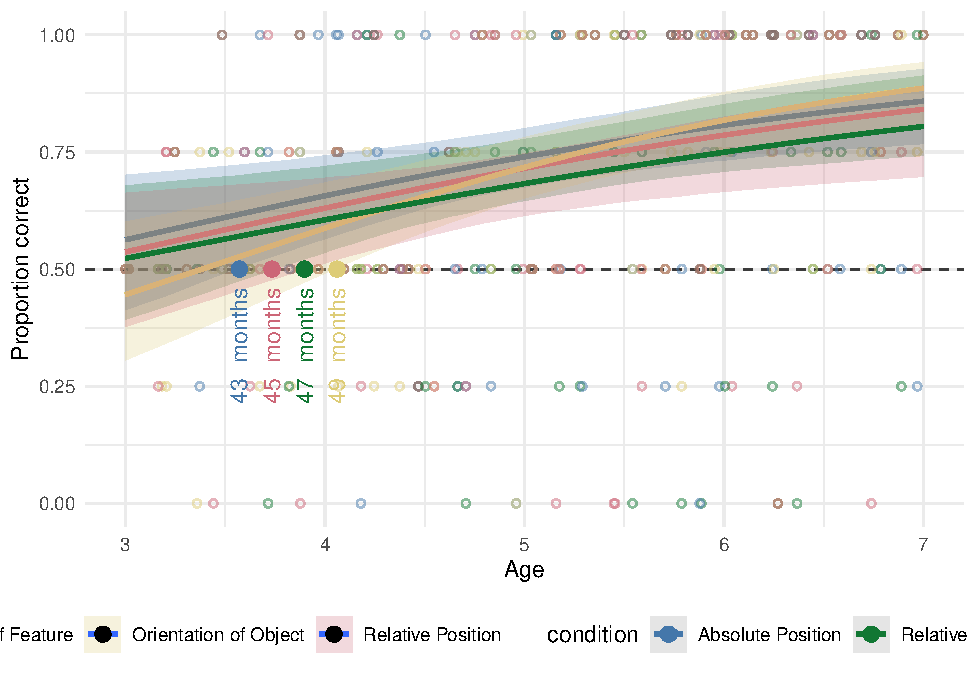
\includegraphics{symlit_rep_manuscript_files/figure-latex/S2_bayes_plot-1.pdf}

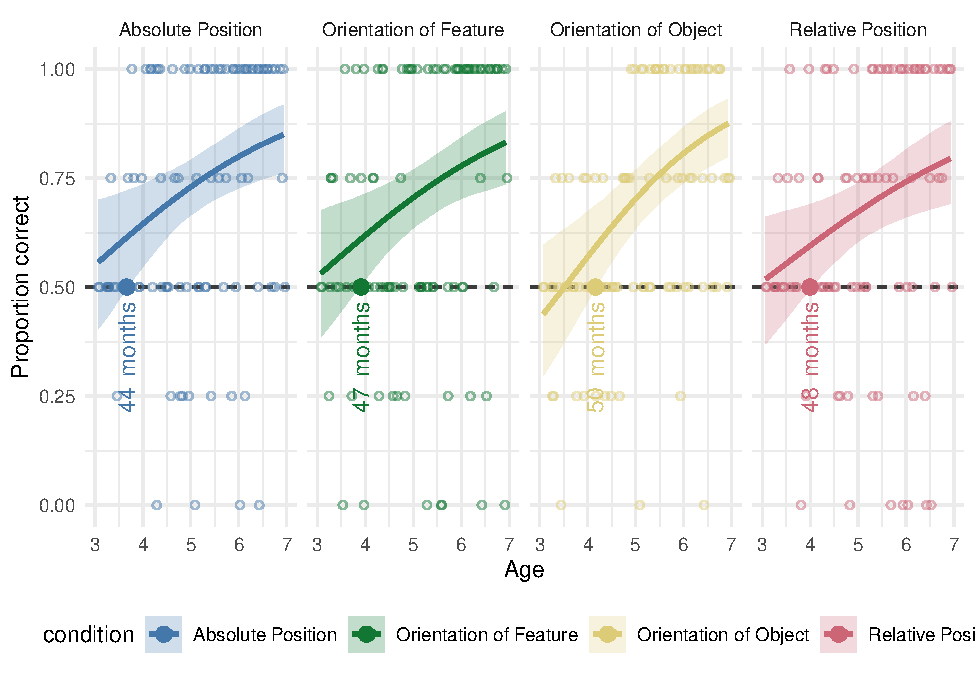
\includegraphics{symlit_rep_manuscript_files/figure-latex/S2_mixbayes_plot-1.pdf}

\subsection{Study 3}\label{study-3}

General note on the aim of the investigation

\subsubsection{Participants}\label{participants-2}

A total of 99 three- to seven-year-old children (M = 59.88 months, SD = 13.44 months, range 36 - 83 months; 55 female) participated. In addition, 23 children (7 female) were tested but excluded for low performance during familiarization (N = 12), for not completing at least eight out of 16 test trials (N = 1), or being fussy (N = 3). Another 4children were excluded due to language problems or technical issues (N = 3).

\subsubsection{Materials}\label{materials-1}

\subsubsection{Analysis}\label{analysis}

Trails
Notation
Model Evaluation

\subsubsection{Results}\label{results-2}

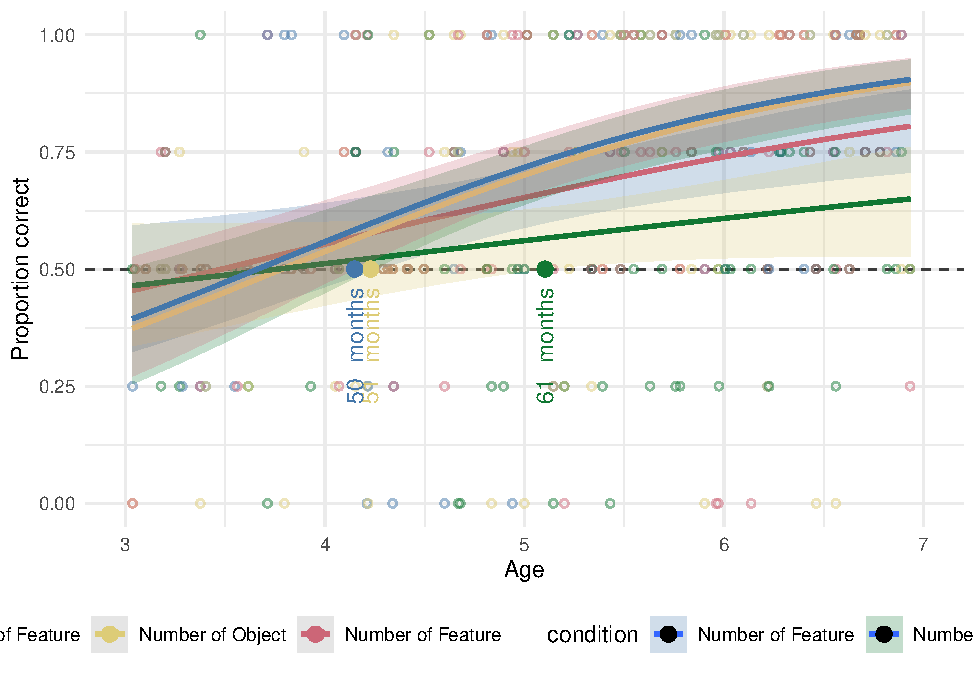
\includegraphics{symlit_rep_manuscript_files/figure-latex/S3_bayes_plot-1.pdf}

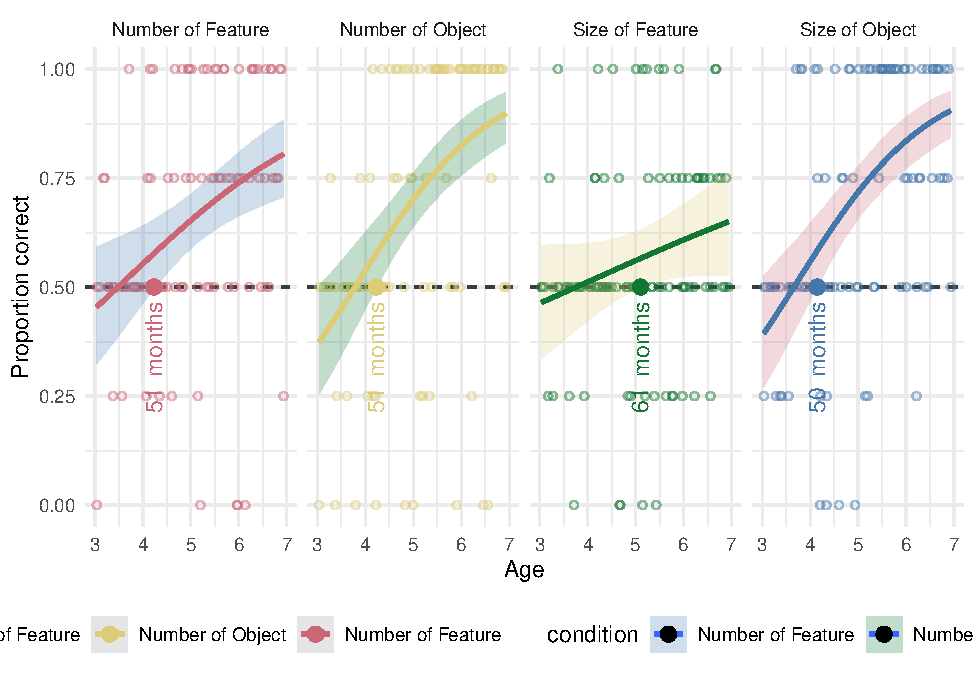
\includegraphics{symlit_rep_manuscript_files/figure-latex/S3_mixbayes_plot-1.pdf}

Lorem ipsum dolor sit amet, consetetur sadipscing elitr, sed diam nonumy eirmod tempor invidunt ut labore et dolore magna aliquyam erat, sed diam voluptua. At vero eos et accusam et justo duo dolores et ea rebum. Stet clita kasd gubergren, no sea takimata sanctus est Lorem ipsum dolor sit amet. Lorem ipsum dolor sit amet, consetetur sadipscing elitr, sed diam nonumy eirmod tempor invidunt ut labore et dolore magna aliquyam erat, sed diam voluptua. At vero eos et accusam et justo duo dolores et ea rebum. Stet clita kasd gubergren, no sea takimata sanctus est Lorem ipsum dolor sit amet.

\section{Additional Analyses}\label{additional-analyses}

possible add-ons
- a model including all conditions
- comparing difficulty across items and tasks
- evaluating manipulations such as complex/simple;
- reaction time analyses

Additional Analyses:

object vs feature
- orfe vs orob
- sife vs siob
- nufe vs nuob

round vs angular
- Study One Study1 - cue A = rund, cue B eckig \ldots if one of them is easier

Reaction Times
just reaction times and perc correct across aged

\section{General Discussion}\label{general-discussion}

Overview

Main Finding

Strengths and Implications

Limitations

\section{Conclusion}\label{conclusion}

Lorem ipsum dolor sit amet, consetetur sadipscing elitr, sed diam nonumy eirmod tempor invidunt ut labore et dolore magna aliquyam erat, sed diam voluptua. At vero eos et accusam et justo duo dolores et ea rebum. Stet clita kasd gubergren, no sea takimata sanctus est Lorem ipsum dolor sit amet.

\newpage

\section{References}\label{references}

\phantomsection\label{refs}
\begin{CSLReferences}{1}{0}
\bibitem[\citeproctext]{ref-bohn2019young}
Bohn, M., Kachel, G., \& Tomasello, M. (2019). Young children spontaneously recreate core properties of language in a new modality. \emph{Proceedings of the National Academy of Sciences}, \emph{116}(51), 26072--26077.

\end{CSLReferences}

\newpage

\appendix


\section{Participants and Exclusions}\label{participants-and-exclusions}

Data collection aimed at testing two children per month of age between the third and seventh birthday for a minimum of 96 children per study. For an overview of the sample distribution, please see figure \ref{fig:suppl-participants-dots}.

\begin{figure}

{\centering 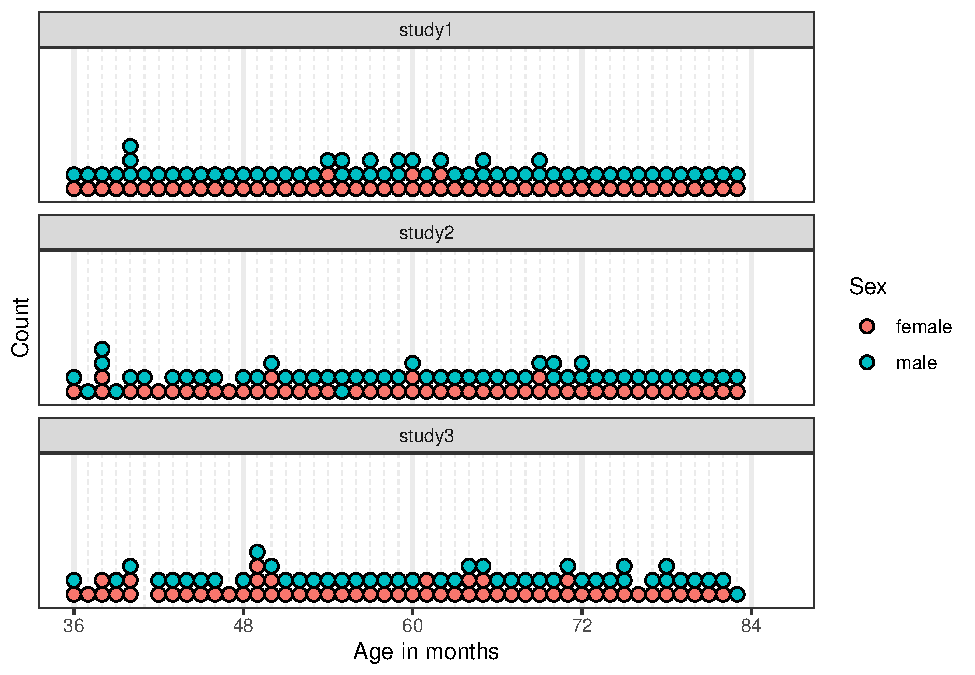
\includegraphics{symlit_rep_manuscript_files/figure-latex/suppl-participants-dots-1} 

}

\caption{Illustration of participants across the age range.}\label{fig:suppl-participants-dots}
\end{figure}

The total number of participants in all three studies comprises XX children. In addition, XX children were tested but not included in the data set due to XXXXXXXX. For an overview of how the respective exclusions are distributed across the age range, please see figure \ref{fig:suppl-drops-dots}. Exclusions due to low performance during familiarization occured almost exclusively between the third and fourth birthday. All other exclusion criteria appear to be randomly distributed across the age range.

\begin{verbatim}
## Warning: The `size` argument of `element_line()` is deprecated as of ggplot2 3.4.0.
## i Please use the `linewidth` argument instead.
## This warning is displayed once every 8 hours.
## Call `lifecycle::last_lifecycle_warnings()` to see where this warning was
## generated.
\end{verbatim}

\begin{figure}

{\centering 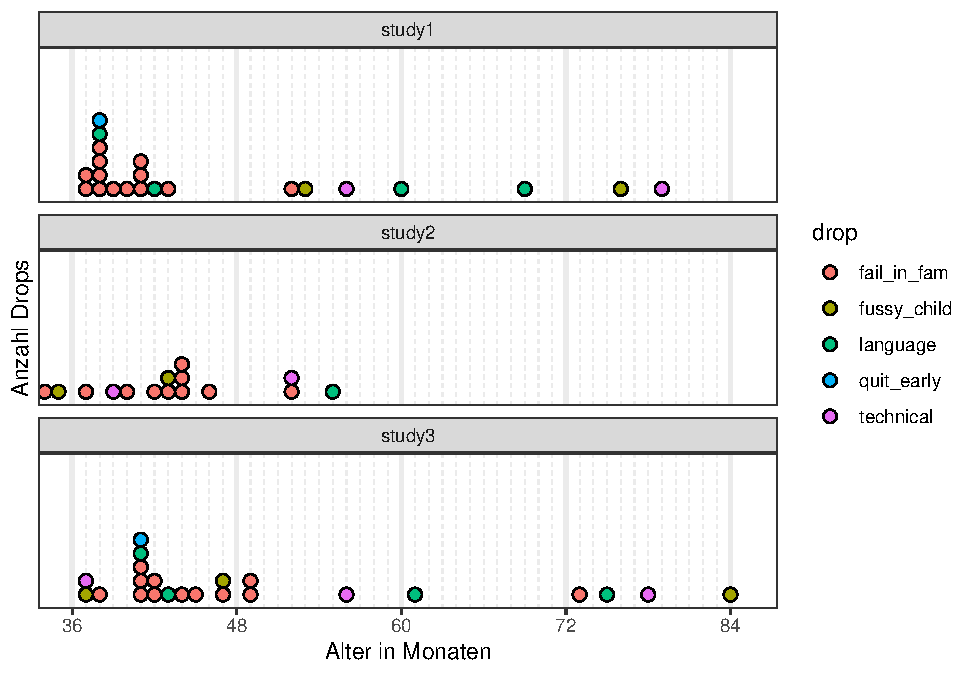
\includegraphics{symlit_rep_manuscript_files/figure-latex/suppl-drops-dots-1} 

}

\caption{Illustration of exclusions across the age range.}\label{fig:suppl-drops-dots}
\end{figure}

\section{Stimulus Material}\label{stimulus-material}

Additional Tables and illustrations for the convenience of the reader. Add illustrations they said; it will add value they said.

\subsection{Study 1}\label{study-1-1}

Additional Tables and illustrations for the convenience of the reader. Add illustrations they said; it will add value they said.

\subsection{Some graphic}\label{some-graphic}

\begin{figure}

{\centering 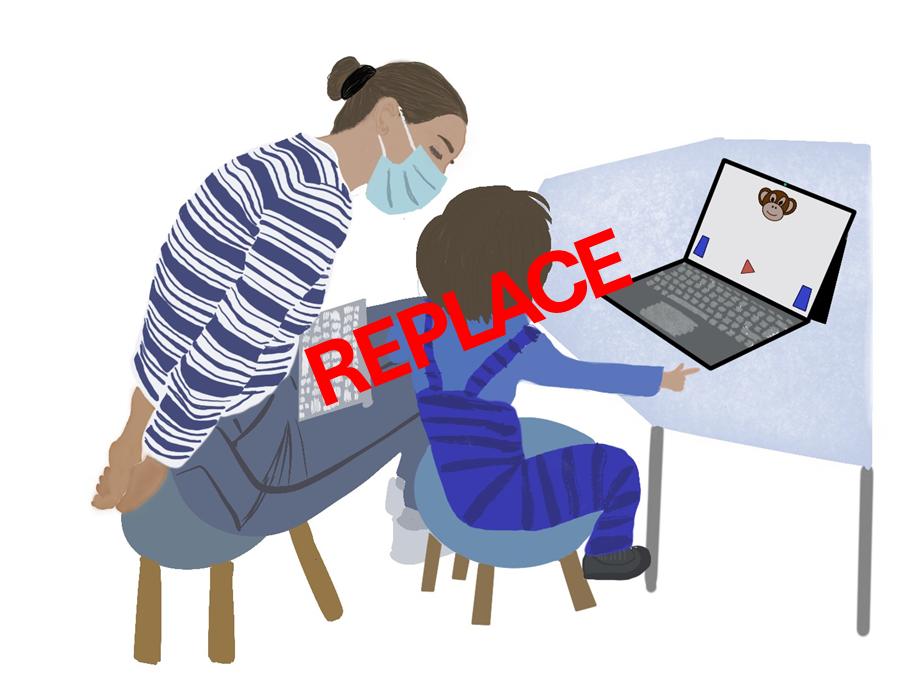
\includegraphics{../illustrations/Symlit_Rep_Setup} 

}

\caption{Check this out}\label{fig:suppl-setup3}
\end{figure}

\subsection{Study 2}\label{study-2-1}

Additional Tables and illustrations for the convenience of the reader. Add illustrations they said; it will add value they said.

\subsection{Some graphic}\label{some-graphic-1}

\begin{figure}

{\centering 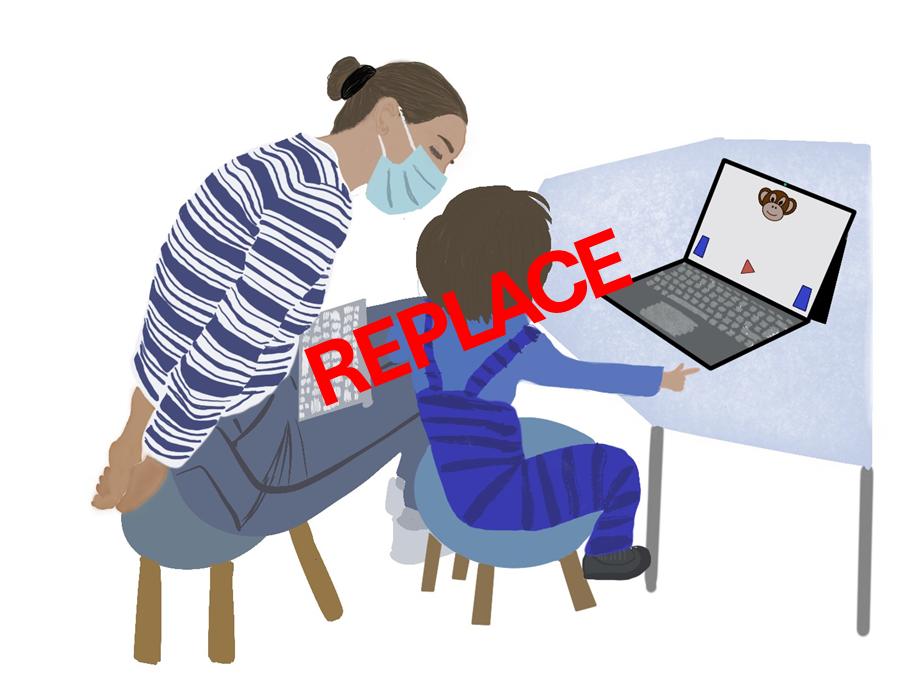
\includegraphics{../illustrations/Symlit_Rep_Setup} 

}

\caption{Check this out}\label{fig:suppl-setup4}
\end{figure}

\subsection{Study 3}\label{study-3-1}

Additional Tables and illustrations for the convenience of the reader. Add illustrations they said; it will add value they said.

\subsection{Some graphic}\label{some-graphic-2}

\begin{figure}

{\centering 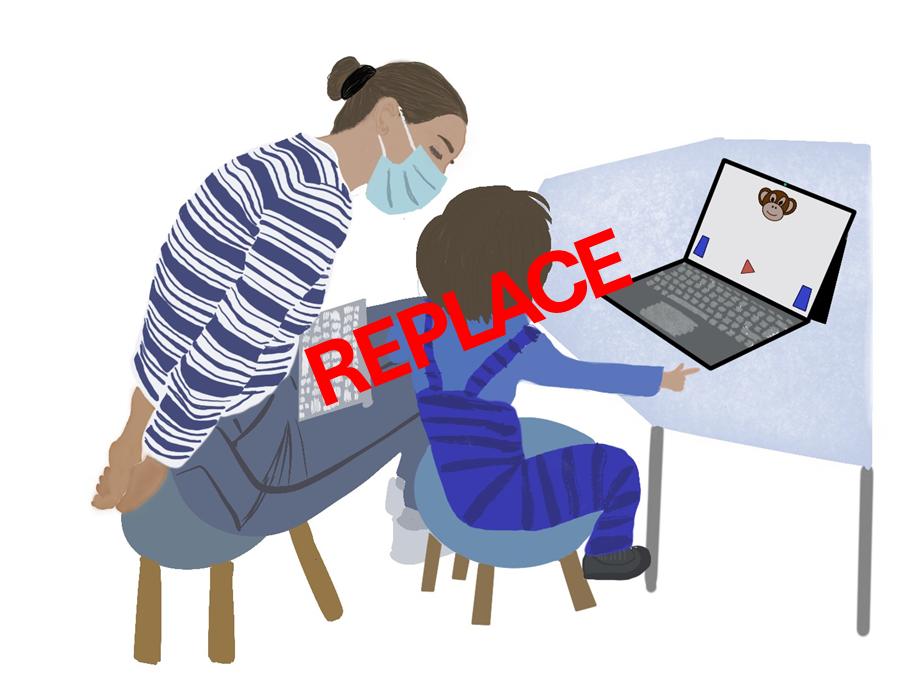
\includegraphics{../illustrations/Symlit_Rep_Setup} 

}

\caption{Check this out}\label{fig:suppl-setup5}
\end{figure}

\section{Descriptive Statistics}\label{descriptive-statistics}

Additional Tables and illustrations for the convenience of the reader. Add illustrations they said; it will add value they said.

\subsection{Study 1}\label{study-1-2}

Additional Tables and illustrations for the convenience of the reader. Add illustrations they said; it will add value they said.

\subsection{Study 2}\label{study-2-2}

Additional Tables and illustrations for the convenience of the reader. Add illustrations they said; it will add value they said.

\subsection{Study 3}\label{study-3-2}

Additional Tables and illustrations for the convenience of the reader. Add illustrations they said; it will add value they said.


\end{document}
